\subsection{\asvn}
\label{section:outils_svn}

\asvn\footnote{\url{http://subversion.apache.org/}} est un système \aos\ de gestion de versions : pour une arborescence donnée, le but est de conserver toutes les versions des fichiers ainsi que les différences entre celles-ci. Pour cela, les différents états successifs de l'arborescence, appelés \emph{révisions}, sont choisis arbitrairement par l'utilisateur au fur et à mesure de leur évolution. Chaque révision est identifiée par un numéro, qui est incrémenté de un par rapport à celui de la révision précédente.

\asvn\ suit un modèle client-serveur illustré en figure~\ref{figure:outils_svn_client-serveur} . En effet, le serveur, appelé \emph{dépôt}, contient l'arborescence de référence. Plusieurs clients peuvent récupérer leur version locale de l'architecture présente sur le dépôt, appelée \emph{copie de travail}. Les différentes copies de travail évoluent indépendamment les unes des autres, tout en restant synchronisées individuellement avec le dépôt. Ainsi, quand on veut sauver une révision d'une copie de travail, celle-ci est soumise au dépôt, et doit être cohérente avec l'état courant de ce dernier. La révision ajoutée pourra alors être récupérée à la demande sur les autres copies de travail. Dans le cas où une copie de travail récupère une révision du dépôt qui concerne des fichiers modifiés localement, \asvn\ gère lui-même le conflit par une fusion (et non pas par un écrasement), et l'intervention de l'utilisateur n'est pas toujours nécessaire.

\begin{figure}
	\centering
	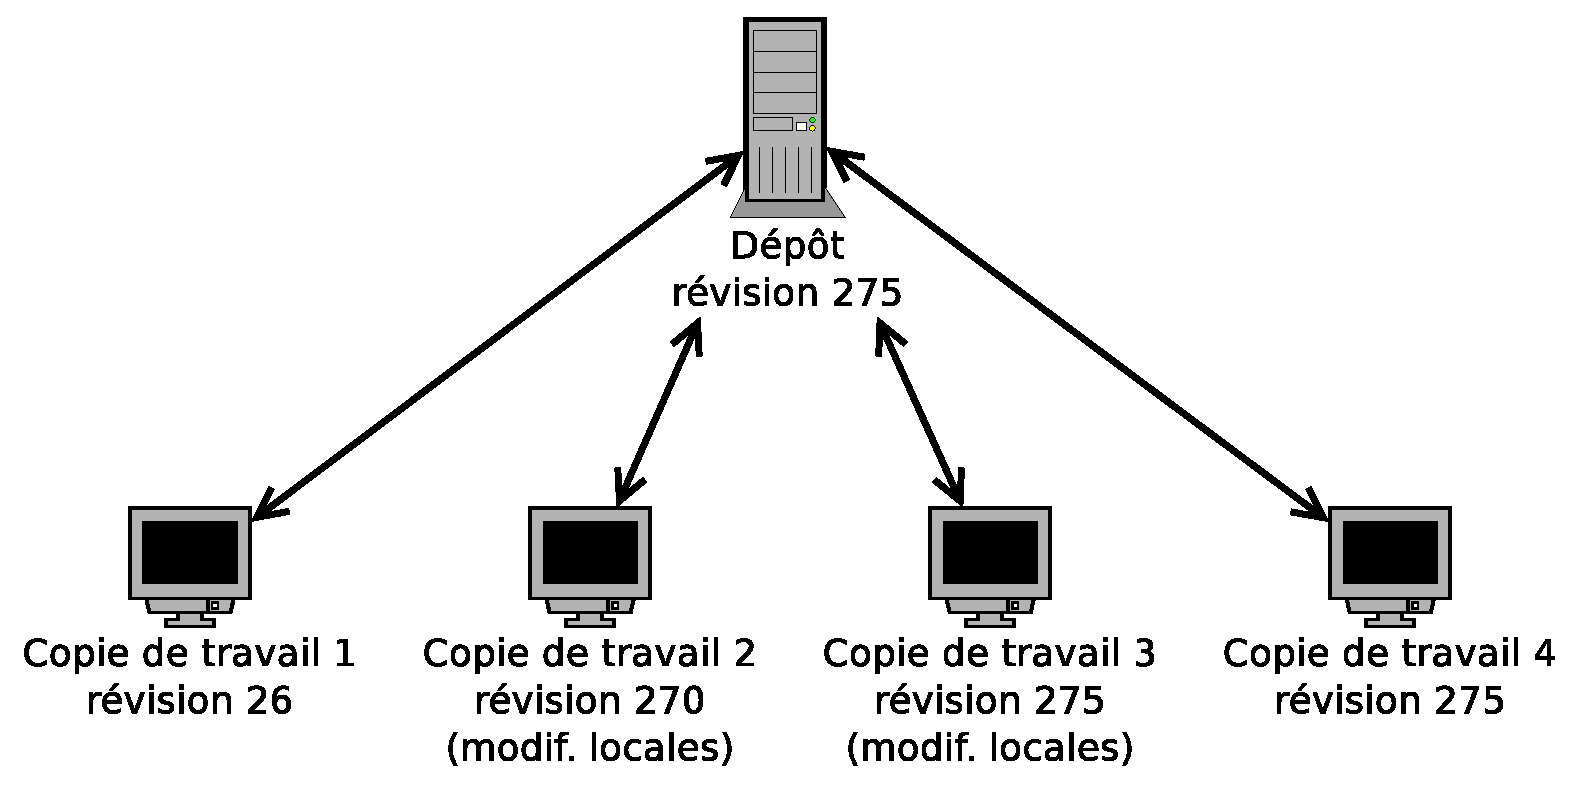
\includegraphics[scale=0.4]{outils_svn_client-serveur}
	\caption{Modèle client-serveur de \asvn}
	\label{figure:outils_svn_client-serveur}
\end{figure}

Chez \asl, \asvn\ est utilisé pour garder un historique complet des codes source développés. En fait, chaque projet dispose de son propre dépôt. À partir de celui-ci, chaque développeur récupère sa propre copie de travail. Dès qu'il a implémenté une fonctionnalité, il l'envoie sous forme de révision au dépôt, et la met ainsi à la disposition de tous. Au delà du partage de code, \asvn\ offre la possibilité aux développeurs de revenir à une version précédente de leurs fichiers, au cas où ils se rendraient compte d'une erreur : de cette façon, plusieurs heures de travail peuvent parfois être sauvées.
